\newpage
\subsection{Cache}

\ifbook{
%--  \begin{figure}[hb]
%--    \begin{center}
%--      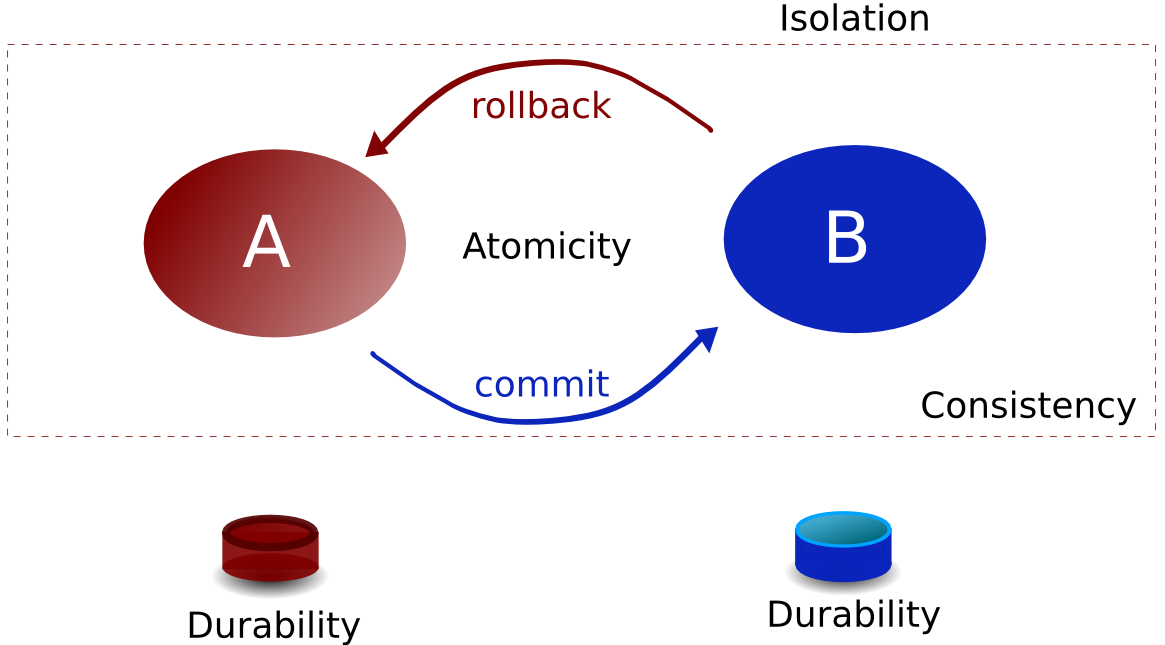
\includegraphics[scale=0.4]{img/transaction.png}
%--      \caption{Caractéristique d'une transaction}
%--      \label{tx}
%--    \end{center}
%--  \end{figure}
%--}
%--
%--\ifslide{
%--  \begin{frame}{Transaction}
%--   \begin{center}
%--     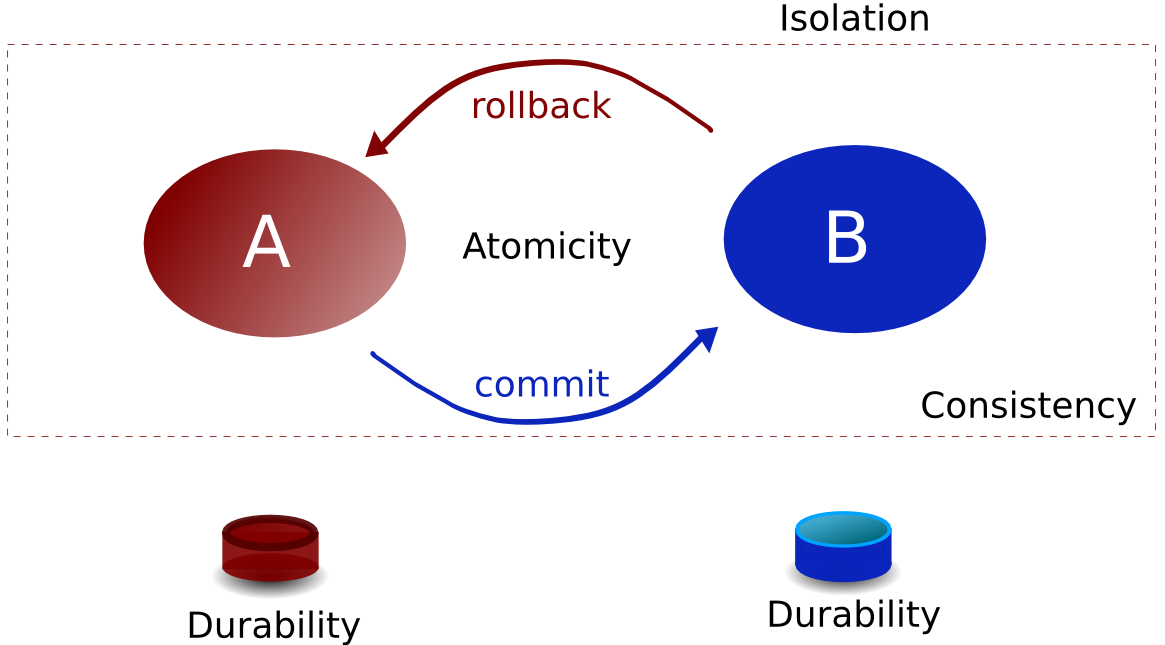
\includegraphics[scale=0.3]{img/transaction.png}
%--   \end{center}
%--  \end{frame}

\paragraph{}

- cache "über alles"\\
- cache DNS
- cache http
- session est un cache !
- cache SQL (Hibernate)
- niveau de cache
- statégie de cache

}
